\Object{Evénement}
{
Un objet de type événement mémorise le signal marquant qu'une condition 
est devenue vraie. Il permet la signalisation entre deux tâches - cela 
implique qu'il y a une tâche émettrice et une tâche destinataire. 
}

{
\begin{enumerate}
   \item Un événement est spécifique à une tâche, susceptible de l'attendre.
   Une tâche est en attente du signal alors qu'une autre sera chargée de l'envoyer. 
   On a donc un producteur et un consommateur.
   \item Une tâche dispose d'un nombre fini d'événements qu'elle peut
   attendre.
   \item L'association des événements aux tâches ne nécessite aucune file
   d'attente : elle fournit donc un mécanisme élémentaire ce qui permet de 
   construire des mécanismes de synchronisation de haut niveau et rend l'objet très efficace.
   \item L'objet événement permet de gérer la signalisation simple (attente
   d'un unique évènement) mais aussi certains cas de signalisation multiple : attente d'un évènement 
   parmi plusieurs (séparés par des OU) ou de plusieurs (séparés par des ET). 
   Les cas plus complexes de signalisation multiple (tels la combinaison de ET
   et de OU) peuvent être gérés en implémentant une agence dédiée.
   \item En combinant l'objet événement à l'agence Horlogerie on pourrait
   gérer des attentes avec délai comme des time-out.
\end{enumerate}
}
{
\begin{enumerate}
   \item \textbf{boolean ARRIVE (listeEvenements, operateur)}
	~\\ - Utile pour la signalisation multiple, cette primitive permet de
	vérifier si les éléments de la liste ListeEvenements sont arrivés en tenant
	compte s'ils sont séparés par des opérateurs OU ou ET (les valeurs possibles
	du paramètre \textit{opérateur}).
   \item \textbf{void ATTENDRE (listeEvenements, operateur)}
	~\\ - La tâche appelante se met dans l'état \textit{en attente}
	 (sous le contrôle de l'ordonnanceur) si les événements de la liste
	 \textit{listeEvenements} ne sont pas arrivés. 
	 Le paramètre \textit{operateur} peut prendre les valeurs ET ou OU et 
	 permet de spécifier si tous les événements de la liste
	 \textit{listeEvenements} sont attendus ou juste un seul d'entre eux. 
	 Dès que les événements nécéssaires sont arrivés, la tâche passe à l'état
	 \textit{prêt} et on appelle l'ordonnaceur.
   \item \textbf{void EFFACER (listeEvenements)}
	~\\ - Tous les événements de la liste \textit{listeEvenements} sont
		mis dans l'état \textit{NON ARRIVé}.
	\item \textbf{void SIGNALER (idEvenement, idTache)}
	~\\ - L'événement qui a l'identifiant \textit{idEvenement} est mis dans l'état
	\textit{ARRIVé} quelque soit sont état initial. 
	Si la tâche réceptrice est dans l'état \textit{en attente} et qu'elle n'attend
	plus d'événement, elle passe à l'état \textit{prêt} et l'ordonnanceur est invoqué. 
	Sinon, l'arrivée de l'évènement est mémorisée et l'état de la tâche ne change pas.
\end{enumerate}
}
{
Les deux états dans lesquels un événement peut se trouver sont \textit{NON
ARRIVé} et \textit{ARRIVé}.

\begin{figure} [htp]
\centering
%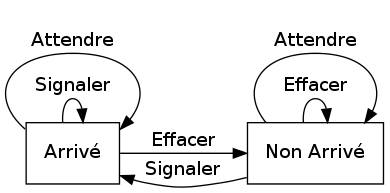
\includegraphics{img/etatEvenement.png}
\end{figure}
}
